\chapter{The Haero Driver}
\labelchapter{driver}

The standalone driver program, \texttt{haero\_driver}, provides a simple way to
explore the capabilities of Haero. It's a simple single-column model with a
bundled one-dimensional dynamics package. With it, you can

\begin{itemize}
  \item run single-column aerosol simulations
  \item perform statistical analysis on ensembles consisting of several columns
  \item conduct time-step convergence studies to build confidence in Haero's
        mathematical algorithms and their implementations
  \item select specific aerosol processes and parametrizations to examine
        in isolation, to debug or verify a given algorithm
  \item study how the aerosol processes interact with one-dimensional dynamics
        and other simplified physical process representations
\end{itemize}

In this chapter we describe the driver and its capabilities. The input format
for the driver is based on YAML and is described in \refappendix{driver_input}.

\section{Column Dynamics}

We use a one-dimensional (vertical) atmosphere and tests of increasing complexity.

Let $z=z(a,t)$ denote the trajectory of the particle labeled $a$ that arrives at physical position $z$ at time $t$.
The label $a$ is the Lagrangian, or material, coordinate. 
Particle trajectories are defined by
\begin{equation}\label{eq:traj}
\deriv{z}{t}(a,t) = w(z(a,t),t),
\end{equation}
where $w(z,t)$ is the vertical velocity.  
In the following sections, it will be convenient to formulate \eqref{eq:traj} in terms of the geopotential $\phi(a,t) = gz(a,t)$, 
\begin{equation}\label{eq:geo_traj}
  \deriv{\phi}{t}(a,t) = gw\left(\frac{\phi(a,t)}{g},t\right).
\end{equation}


Adiabatic column dynamics are described by the 1D Euler equations for a moist atmosphere,
\begin{subequations}\label{eq:1d}
  \begin{align}
    \totd{w} &= -g\left(\frac{1}{\rho}\partd{p}{\phi} + 1\right), \label{eq:momentum}\\
    \totd{\rho} &= - g\rho \partd{w}{\phi}, \label{eq:continuity}\\
    \totd{\theta_v} &= 0, \label{eq:thermo},\\
    \totd{q_v} &= 0, \label{eq:qv}
  \end{align}
\end{subequations}
where $\rho$ is density, $p$ is pressure, $\theta_v$ is the virtual potential temperature, and $q_v$ is the water vapor mass mixing ratio.
As in \cite{Taylor2020}, we treat virtual potential temperature $\theta_v$ as a material invariant.
The momentum, continuity, thermodynamic equation, and transport equation (respectfully) combine with \eqref{eq:geo_traj} and the equation of state,
\begin{equation}\label{eq:eos}
  \frac{p}{\Pi} = \rho R \theta_v,
\end{equation}
to define the complete system.
Above, $\Pi = (p/p_{ref})^{\kappa}$ is the nondimensional Exner pressure, with constant $\kappa = R/c_p$, where $R$ is the dry air gas constant and $c_p$ is the specific heat of dry air at constant pressure.
We have 6 prognostic variables: $\phi, w, \rho, \theta_v, q_v, p$, and 6 equations in \eqref{eq:geo_traj}, \eqref{eq:1d}, \eqref{eq:eos}.
The boundary conditions are $w(0,t) = w(z_{top},t) = 0$.

The advantage of the Lagrangian frame of reference imposed by \eqref{eq:geo_traj} is that the material derivative becomes an ordinary time derivative, $D/Dt = d/dt$. 
Hence, for the remainder of this note we simply use $d/dt$ in our notation.

We begin with an ansatz that the velocity has a simple form,
\begin{equation}\label{eq:z_vel}
  w(z,t) = w_0\sin\frac{\pi z}{z_{top}}\sin \frac{2\pi t}{t_p},
\end{equation}
where we have introduced parameters for the maximum velocity, $w_0$, the top of the model column, $z_{top}$, and the period of oscillation $t_p$.  
This velocity satisfies the boundary conditions and the initial condition, $w(z,0) = 0$.
We assume that this velocity is valid for all time throughout the whole column, from $z=0$ to $z=z_{top}$.
In terms of the geopotential, \eqref{eq:z_vel} becomes,
\begin{equation}\label{eq:phi_vel}
  w(\phi,t) = w_0 \sin \frac{\pi \phi}{g z_{top}}\sin\frac{2\pi t}{t_p}.
\end{equation}
Since velocity is prescribed, it does not need to be prognosed. 
This eliminates \eqref{eq:momentum} from our system of equations \eqref{eq:1d}.
Our goal is to derive the other variables associated with 1D motion in a non-hydrostatic column so that we have consistent dynamics and thermodynamics.

Substituting \eqref{eq:phi_vel} in \eqref{eq:geo_traj} we discover a separable ODE,
\begin{align}
  \deriv{\phi}{t} &= gw_0\sin\frac{\pi \phi}{g z_{top}}\sin\frac{2\pi t}{t_p},\\
  \Rightarrow \int \csc\frac{\pi \phi}{g z_{top}}\,d\phi &= g w_0\int\sin\frac{2\pi t}{t_p}\,dt,
\end{align}
whose solution is
\begin{equation}\label{eq:phi_sol}
\phi(t) = \frac{2gz_{top}}{\pi}\arctan\left[\tan\frac{\pi \phi_0}{2g z_{top}}\exp\left(\frac{w_0t_p}{z_{top}} \sin^2 \frac{\pi t}{t_p}\right)\right].
  \end{equation}

\begin{figure}[H]
  \centering
  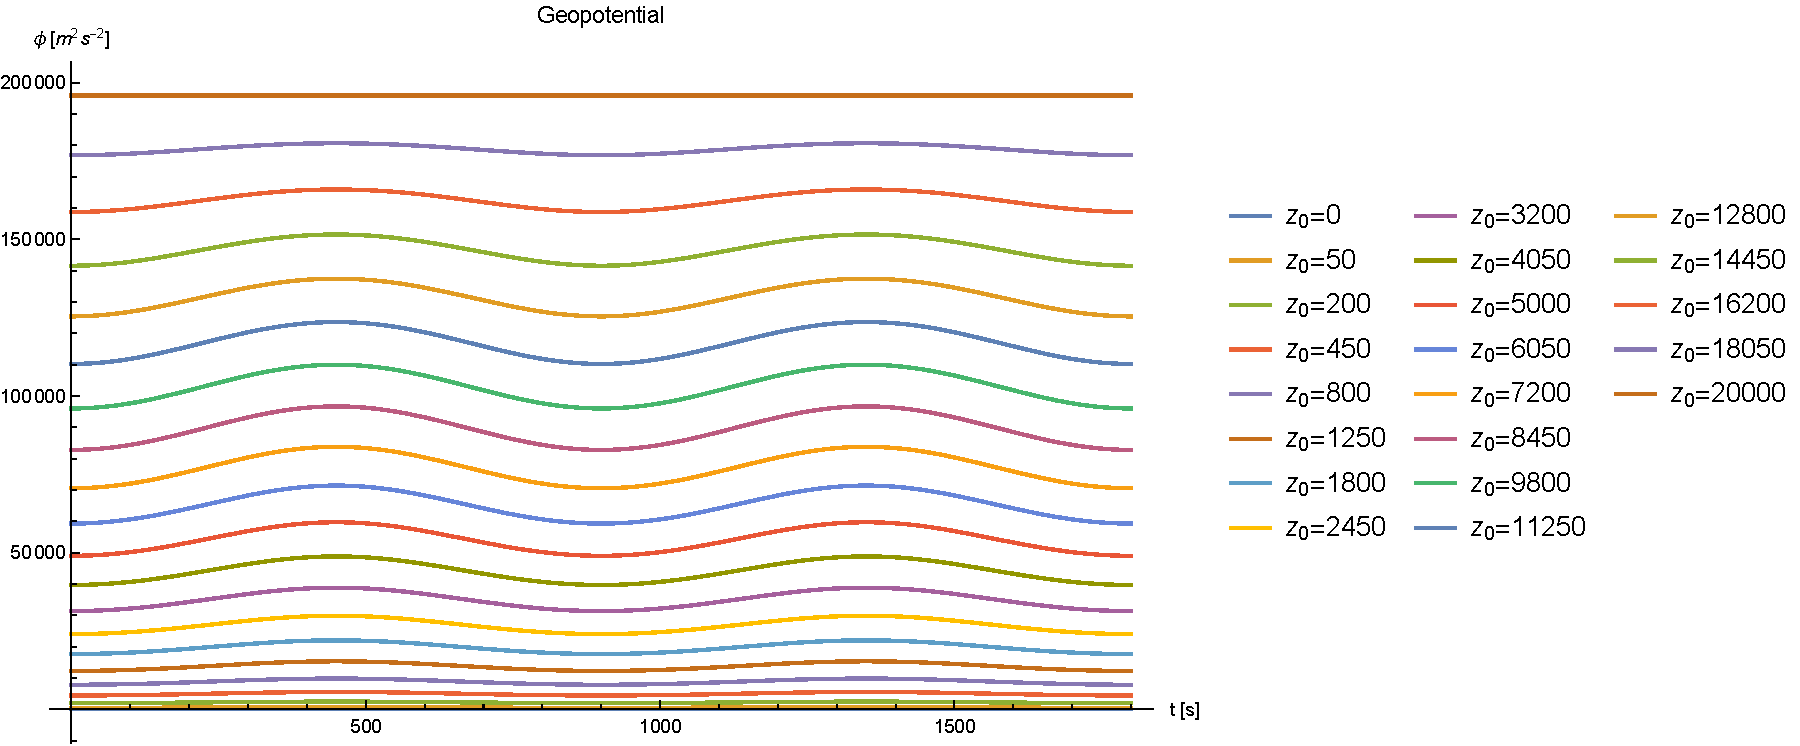
\includegraphics[width=\linewidth]{figures/geopotential_plot}
  \caption{Geopotential $\phi(t)$ for $\phi_0 = gz_0$ and $z_0$ values listed in the legend, with parameters $w_0=5$, $T_{v0}=300$, $\Gamma_v=0.01$, $z_{top}=20000$, $t_p=900$.}\label{fig:geopotential}
\end{figure}

We use \eqref{eq:phi_vel} to find the divergence, which is required by the continuity equation \eqref{eq:continuity},
\begin{equation}\label{eq:div}
  \partd{w}{\phi}(\phi,t) = \frac{\pi w_0}{g z_{top}}\cos\frac{\pi \phi(t)}{gz_{top}}\sin\frac{2\pi t}{t_p}.
\end{equation}
Substituting \eqref{eq:div} into \eqref{eq:continuity}, we find another separable ODE:
\begin{align*}
  \deriv{\rho}{t} &= -\rho \left(\frac{\pi w_0}{z_{top}}\cos\frac{\pi \phi(t)}{g z_{top}}\sin\frac{2\pi t}{t_p}\right)\\
  \Rightarrow \int \frac{1}{\rho}\,d\rho &= -\frac{\pi w_0}{z_{top}}\cos\frac{\pi \phi(t)}{z_{top}}\int \sin \frac{2\pi t}{t_p}\,dt.
\end{align*}
The solution is
\begin{align}\label{eq:density}
  \rho(\phi(t),t) = \rho_0(\phi_0)\exp\left[\frac{ w_0 t_p}{2z_{top}}\left(\cos\frac{\pi {\phi}(t)}{gz_{top}}\cos\frac{2\pi t}{t_p}-\cos\frac{\pi {\phi_0}}{gz_{top}}\right)\right].
\end{align} 

\begin{figure}[H]
  \centering
  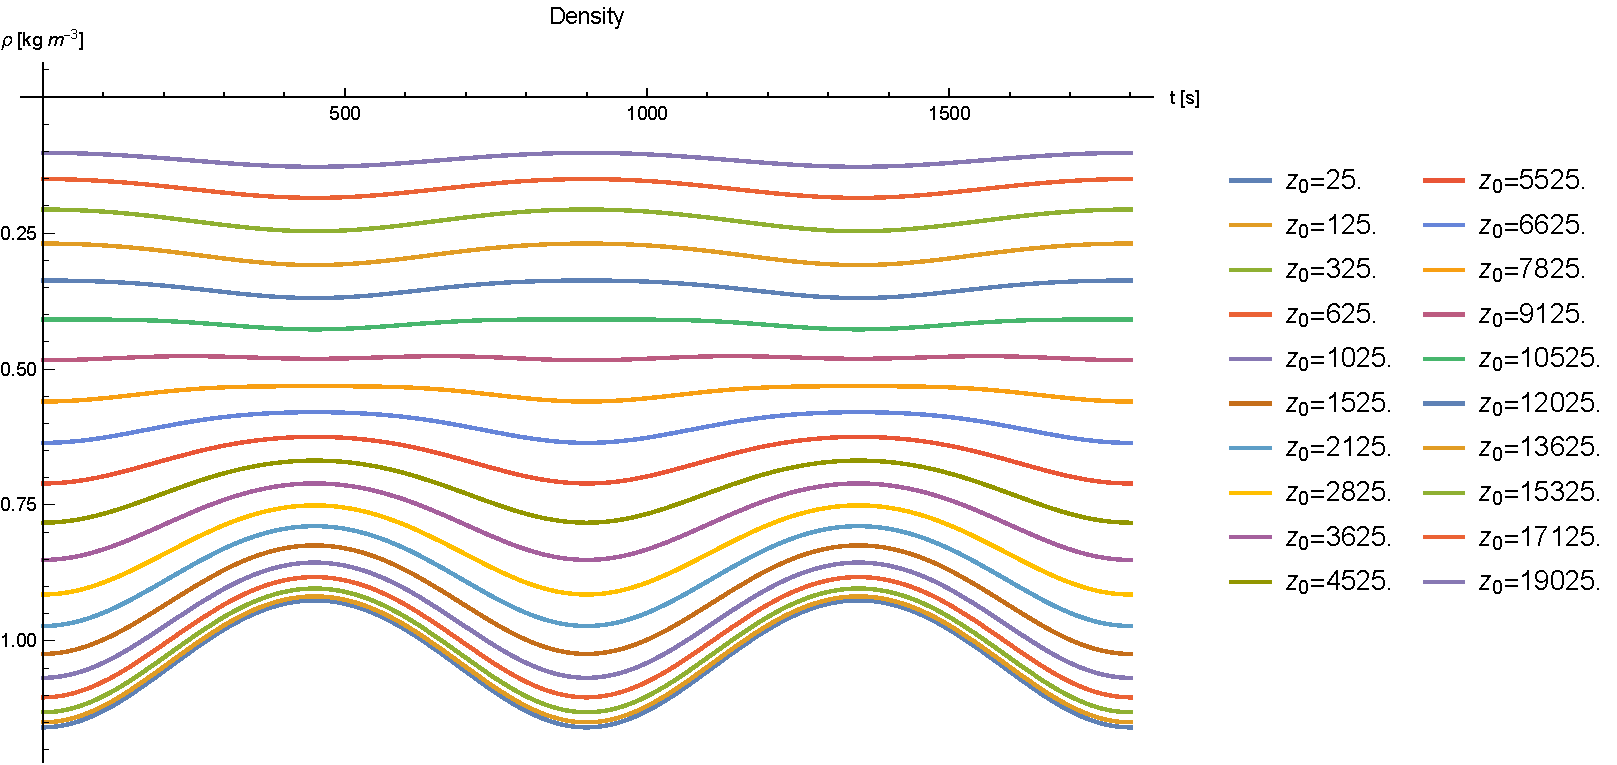
\includegraphics[width=\linewidth]{figures/density_plot}
  \caption{Density $\rho(\phi(t),t)$ for $\phi_0 = gz_0$ and $z_0$ values listed in the legend, with parameters $w_0=5$, $T_{v0}=300$, $\Gamma_v=0.01$, $z_{top}=20000$, $t_p=900$.}\label{fig:density}
\end{figure}

To find the pressure, we use \eqref{eq:density} in \eqref{eq:eos},
\begin{align}
  \frac{p}{\Pi} &= R\rho(\phi(t),t)\theta_v(\phi(t),t),\notag \\
  p(\phi(t),t) &= \left(p_{ref}^{-\kappa} R \rho(\phi(t),t)\theta_v(\phi(t),t)\right)^{1/(1-\kappa)}.\label{eq:pressure}
\end{align}

\begin{figure}[H]
  \centering
  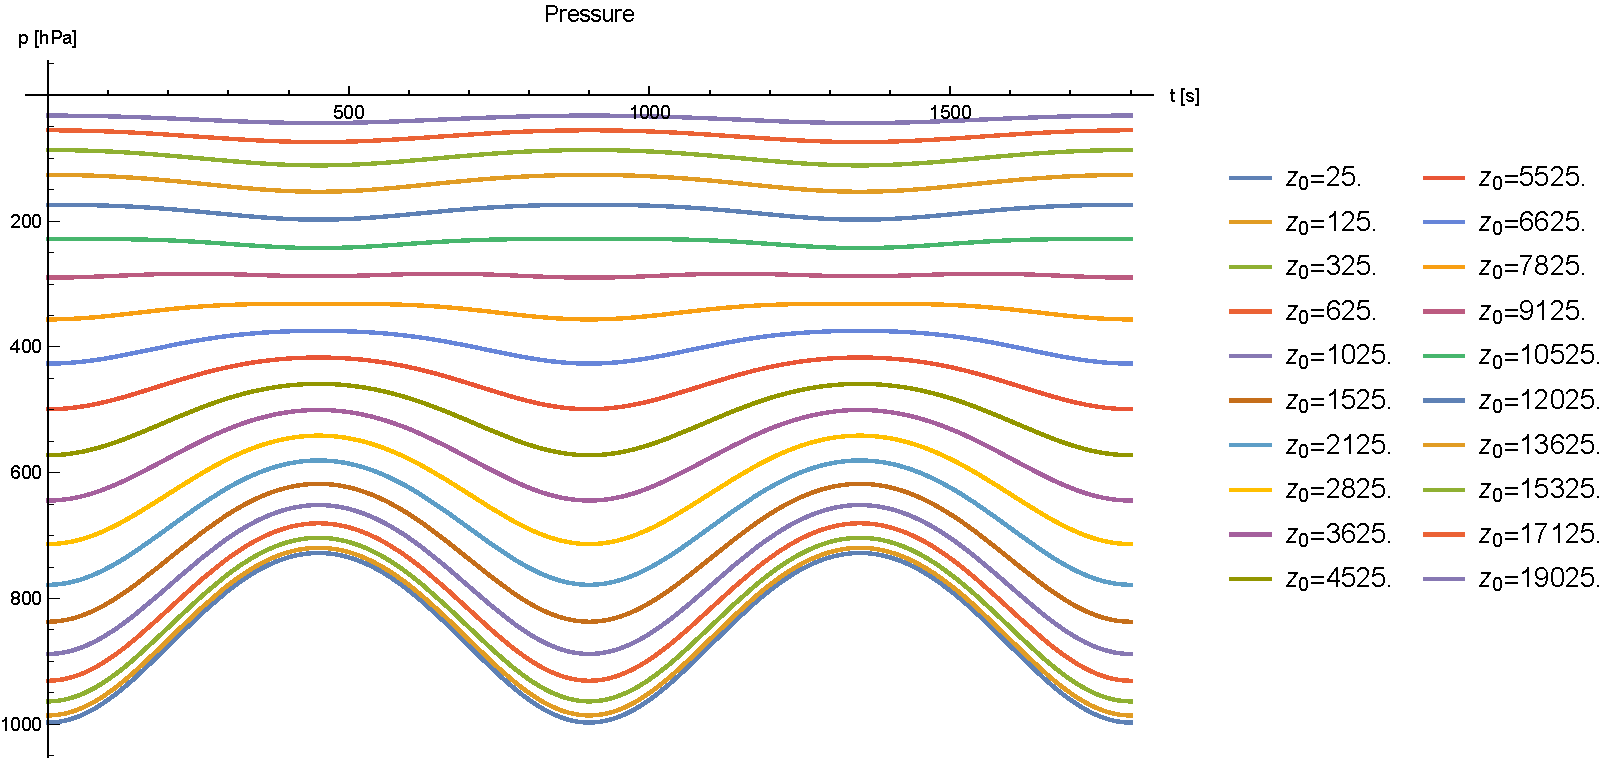
\includegraphics[width=\linewidth]{figures/pressure_plot}
  \caption{Pressure $p(\phi(t),t)$ for $\phi_0 = gz_0$ and $z_0$ values listed in the legend, with parameters $w_0=5$, $T_{v0}=300$, $\Gamma_v=0.01$, $z_{top}=20000$, $t_p=900$.}\label{fig:pressure}
\end{figure}

\subsection{Physical interpretation}

Physically, the ansatz \eqref{eq:z_vel} may be interpreted via \eqref{eq:momentum} as defining the balance between buoyancy, the pressure gradient force, and gravity to be,
\begin{align}
  -g\left(1 +  \frac{1}{\rho}\partd{p}{\phi}\right) &= \deriv{w}{t}(\phi,t), \notag \\
  &= \frac{2\pi w_0}{t_p}\sin\frac{\pi\phi}{gz_{top}}\cos\frac{2\pi t}{t_p} + \frac{\pi w_0^2}{2z_{top}}\sin\frac{2\pi\phi}{gz_{top}}\sin^2\frac{2\pi t}{t_p},
\end{align}
where the right-hand side is the time derivative of \eqref{eq:phi_vel}.
It is most straightforward to derive this interpretation by decomposing the pressure into a constant, hydrostatically balanced reference state with a superimposed perturbation \cite{Klemp1978,Srivastava1967,SoongOgura1973} so that $p = \overline{p} + p'$.
Combining this decomposition (and similar treatment of temperature and density) with the equation of state leads to a formulation of the total pressure gradient as the background hydrostatic balance plus a perturbation due to nonhydrostatic buoyancy.  
In \cite{Klemp1978,Srivastava1967,SoongOgura1973} this arises as quadratic terms of the perturbation variables are neglected.  
It is interesting that a similar (though not equivalent\footnote{Taylor et.~al.~\cite{Taylor2020} retain the full form of the pressure gradient, without a linearization.}) term arises in \cite{Taylor2020} as a result of the choice of a vertical mass coordinate based on hydrostatic pressure.
  
\subsection{Initialization}

Initial conditions are defined by stationary, $w(\phi(0),0) = 0,$ hydrostatic balance with a constant lapse rate in the virtual temperature profile, and exponential decay in the water vapor mixing ratio.

The initial virtual temperature profile is defined by two parameters, $T_{0}$ and $\Gamma_v$ (with default values 300K and 0.01 K/m, respectively),
\begin{equation}\label{eq:tv}
  T_{v0}(z) = T_{0} - \Gamma_v z.
\end{equation}
Using \eqref{eq:tv} with $p=\rho R T_v$, an equivalent form of the equation of state \eqref{eq:eos}, the hydrostatic equation $\partd{p}{z} = -\rho g$, and separation of variables (again), we derive expressions that relate initial height to initial pressure,
\begin{align}
  p_0(z) = \begin{cases}
          p_{ref}\exp\left(\frac{-g z}{R T_{0}}\right) & \Gamma_v = 0,\\[0.5em]
          p_{ref}\, T_0^{-g/(R\Gamma_v)}\left(T_{0} - \Gamma_v z\right)^{g/(R\Gamma_v)} & \Gamma_v \ne 0,
        \end{cases} \label{eq:p_of_z}\\[0.5em]
  z_0(p) = \begin{cases}
         -\frac{R T_{0}}{g}\log\frac{p}{p_{ref}} & \Gamma_v = 0,\\[0.5em]
         \frac{T_{0}}{\Gamma_v}\left(1 - \left(\frac{p}{p_{ref}}\right)^{R\Gamma_v/g}\right) & \Gamma \ne 0.
       \end{cases}\label{eq:z_of_p}
\end{align}
It follows that the initial virtual potential temperature profile is defined as
\begin{equation}
  \theta_{v0}(z) = T_{v0}(z)\left(\frac{p_{ref}}{p_0(z)}\right)^\kappa.
\end{equation}
The initial water vapor mixing ratio profile is also defined by two parameters, $q_0$ and $q_1$, with default values $q_0=0.015$ kg H$_2$O / kg air and $q_1 = $ 1E-3 m$^{-1}$, as
\begin{equation}
  q_{v0}(z) = q_0e^{-q_1 z}.
\end{equation}
Initial densities are defined as
\begin{equation}
  \rho_0(z) = \frac{p_0(z)}{R\,T_{v0}(z)}.
\end{equation}

\subsection{Discretized column}

In the Haero driver, we emulate the vertical grid staggering used by the HOMME-NH dynamical core \cite{Taylor2020}, which has $n_{lev}$ levels and $n_{lev}+1$ interfaces.
Levels are indexed by integer values $k$, for $k=1,\dotsc,n_{lev}$ and interfaces are indexed by $k+1/2$, for $k=0,\dotsc,n_{lev}$.

Geopotential and vertical velocity are defined at interfaces;
\begin{align}
  \phi_{k+1/2}(t) &= \frac{2gz_{top}}{\pi}\arctan\left[\tan\frac{\pi \phi_{k+1/2}(0)}{2g z_{top}}\exp\left(\frac{w_0t_p}{2z_{top}} \sin^2 \frac{2\pi t}{t_p}\right)\right], \label{eq:phi_disc}\\
  w_{k+1/2}(t) &= w_0 \sin \frac{\pi \phi_{k+1/2}(t)}{g z_{top}}\sin\frac{2\pi t}{t_p}. \label{eq:w_disc}
\end{align}

Density, virtual potential temperature, water vapor, and pressure are defined at level midpoints,
\begin{align}
  \rho_k(t) &= \rho_0(\overline{\phi_k}(0))\exp\left[\frac{ w_0 t_p}{2z_{top}}\left(\cos\frac{\pi \overline{\phi_k}(t)}{gz_{top}}\cos\frac{2\pi t}{t_p}-\cos\frac{\pi \overline{\phi_{k}}(0)}{gz_{top}}\right)\right], \label{eq:rho_disc}\\
  \theta_{vk}(t) &= \theta_{v0}(\overline{\phi_k}(0)/g), \label{eq:thetav_disc} \\
  q_{vk}(t) &= q_{v0}(\overline{\phi_k}(0)/g), \label{eq:qv_disc} \\
  % p_k(t) &= \left(p_0^{-\kappa}R \, \rho_k(t)\,\left(\theta_v\right)_k(t)\right)^{1/(1-\kappa)}, 
p_k(t) &=  \left(p_{ref}^{-\kappa} R \rho_k(t)\theta_{vk}(t)\right)^{1/(1-\kappa)}\label{eq:p_disc}
\end{align}
where the constants $g = 9.8$ m/s$^2$, $p_{ref} = 10^5$ Pa, and $\kappa = 0.286$; the overline denotes an average, $\overline{\phi_k}(t) = (\phi_{k-1/2}(t) + \phi_{k+1/2}(t))/2$.



%Column data are initialized as follows:
%\begin{enumerate}
%  \item A set of levels and interfaces are defined in one of two ways:
%  \begin{enumerate}
%    \item Height level interfaces $z_{1/2}, z_{3/2}, \dotsc, z_{n_{lev}+1/2}$  are chosen such that $z_{1/2} = z_{top}$ and $z_{n_{lev}+1/2} = 0$.
%        Geopotential $\phi(z_{i+1/2}) = g z_{i+1/2}$ is defined for $i=0,\dotsc,n_{lev}$.
%    \begin{itemize}
%      \item Level midpoints are initialized so that $z_i = (z_{i+1/2} + z_{i-1/2})/2$ for $i=1,\dotsc,n_{lev}$. 
%      \item Level and interface values for $s$ and $\Delta s$ are computed using \eqref{eq:s_coord}.
%      \item Given a user-specified lapse rate $\Gamma$, hydrostatic pressure $\pi$ is initialized at each level interface and pressure $p$ is initialized at level midpoints using \eqref{eq:hydrostatic_pressure_profile}.
%    \end{itemize}
%    \item Pressure level interfaces $\pi_{1/2}, \pi_{3/2}, \dotsc, \pi_{n_{lev}+1/2}$  are chosen such that $\pi_{1/2} = \pi_{top}$ and $\pi_{n_{lev}+1/2} = p_0$.
%    \begin{itemize}
%      \item Given a user-specified lapse rate $\Gamma$, geopotential $\phi=gz$ is initialized at each level interface using \eqref{eq:hydrostatic_height_profile}.
%      \item Level midpoints are initialized so that $z_i = (z_{i+1/2} + z_{i-1/2})/2$ for $i=1,\dotsc,n_{lev}$, and level \& interface values for $s$ and $\Delta s$ are defined using \eqref{eq:s_coord}.
%      \item Pressure $p$ is defined via \eqref{eq:hydrostatic_pressure_profile} at level midpoints. 
%    \end{itemize}
%  \end{enumerate}
%  \item Pseudodensity is defined at each level midpoint,
%    \begin{equation}
%      \left(\partd{\pi}{s}\right)_i = -\frac{g(\pi_{i+1/2}-\pi_{i-1/2})}{z_{top}(\phi_{i+1/2}-\phi_{i-1/2})},
%    \end{equation}
%    where we have used $\partial s / \partial z = - 1 /z_{top}$ from \eqref{eq:s_coord}.
%%    \begin{rem}
%%    This is an example of the $s$-coordinate cancelling, which is why most models don't explicitly define it.
%%    \end{rem}
%  \item A water vapor profile is defined, by choosing constant values for $q_v^{(0)}$ and $q_v^{(1)}$ in \eqref{eq:qv_profile}, and its values are stored at level midpoints.
%  \item Virtual potential temperature $\theta_v = T_v(p_0/p)^{\kappa}$, with the dry-air constant $\kappa = R_{dry}/c_p$, is defined at level midpoints.
%  \item The initial velocity profile is defined, usually $w=0$.  
%\end{enumerate}

\subsection{Creating a Haero atmosphere}

The above dynamics are motivated by the input requirements of the various parameterizations.  
These are encapsulated by the \texttt{haero::Atmosphere} class, which requires temperature, pressure, height, and relative humidity data. 
We already have pressure and height.
Temperature may be diagnosed using the approximation given by \cite[eq.~(2.3)]{KlempWilhelmson1978},
\begin{equation}
  T_k(t) \approx \frac{\theta_{vk}(t) ~ \Pi_k(t)}{1+\alpha_q ~ q_{vk}(t)},
\end{equation}
with constant $\alpha_q = 0.61$.

\begin{figure}[H]
  \centering
  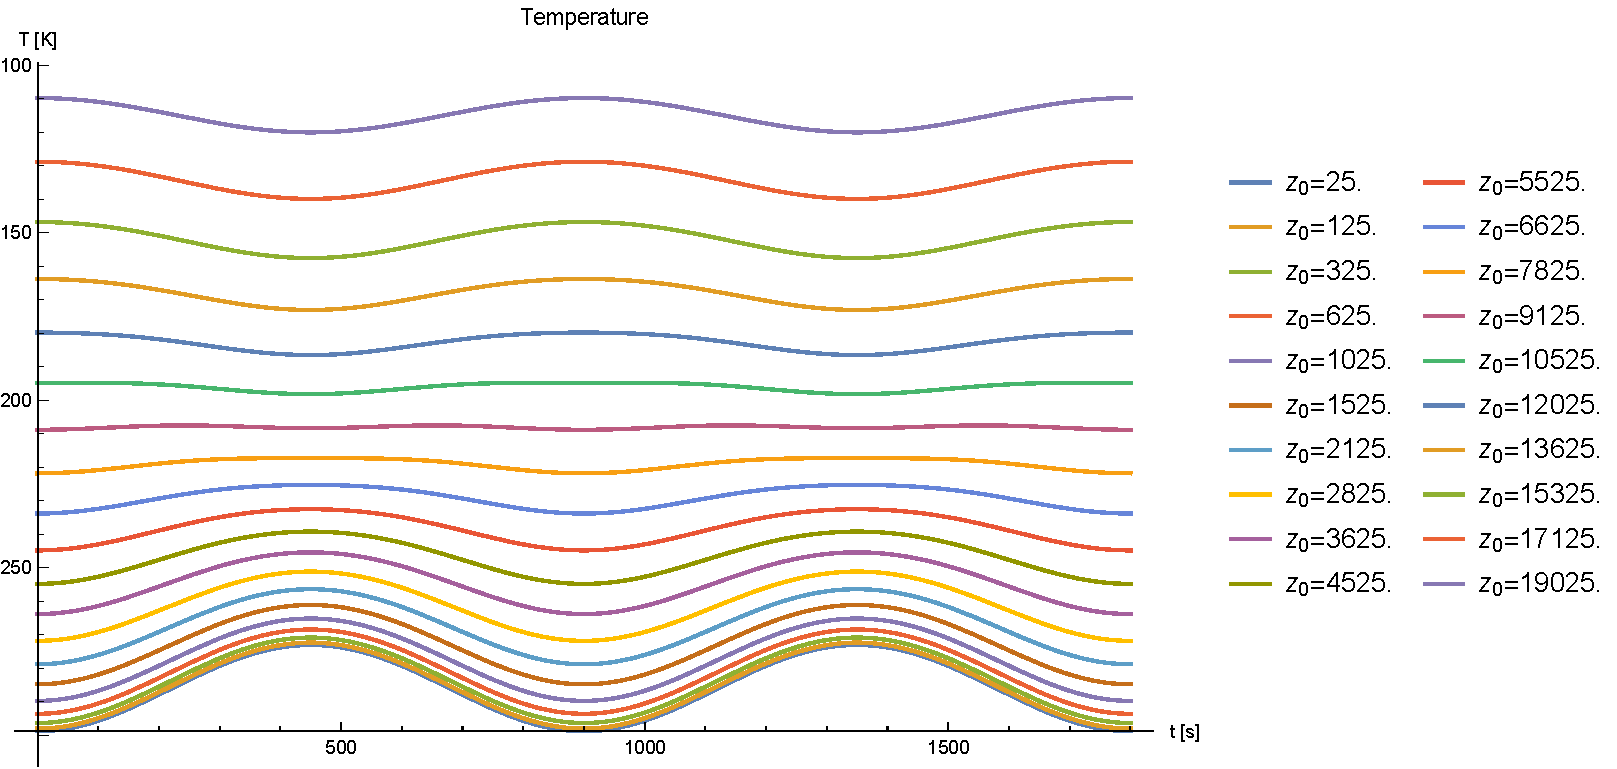
\includegraphics[width=\linewidth]{figures/temperature_plot}
  \caption{Temperature for the same parameters as in Figures \ref{fig:geopotential},\ref{fig:density}, and \ref{fig:pressure}, with the additional parameters $q_{0}=6$E-3, $q_1=2.5$E-3.}\label{fig:temperature}
\end{figure}

We compute relative humidity as $s = q_v/q_{vsat}$, where $q_{vsat}$ is the saturation mixing ratio.
We use the Tetens equation to find $q_{vsat}$ \cite[eqn. (A1)]{SoongOgura1973},
\begin{equation}\label{eq:tetens}
  q_{vs}(T) = \frac{380.042}{p}\exp\left(\frac{15}{2}\log(10) \frac{T-273}{T-36}\right).
\end{equation}

\begin{figure}[H]
\centering
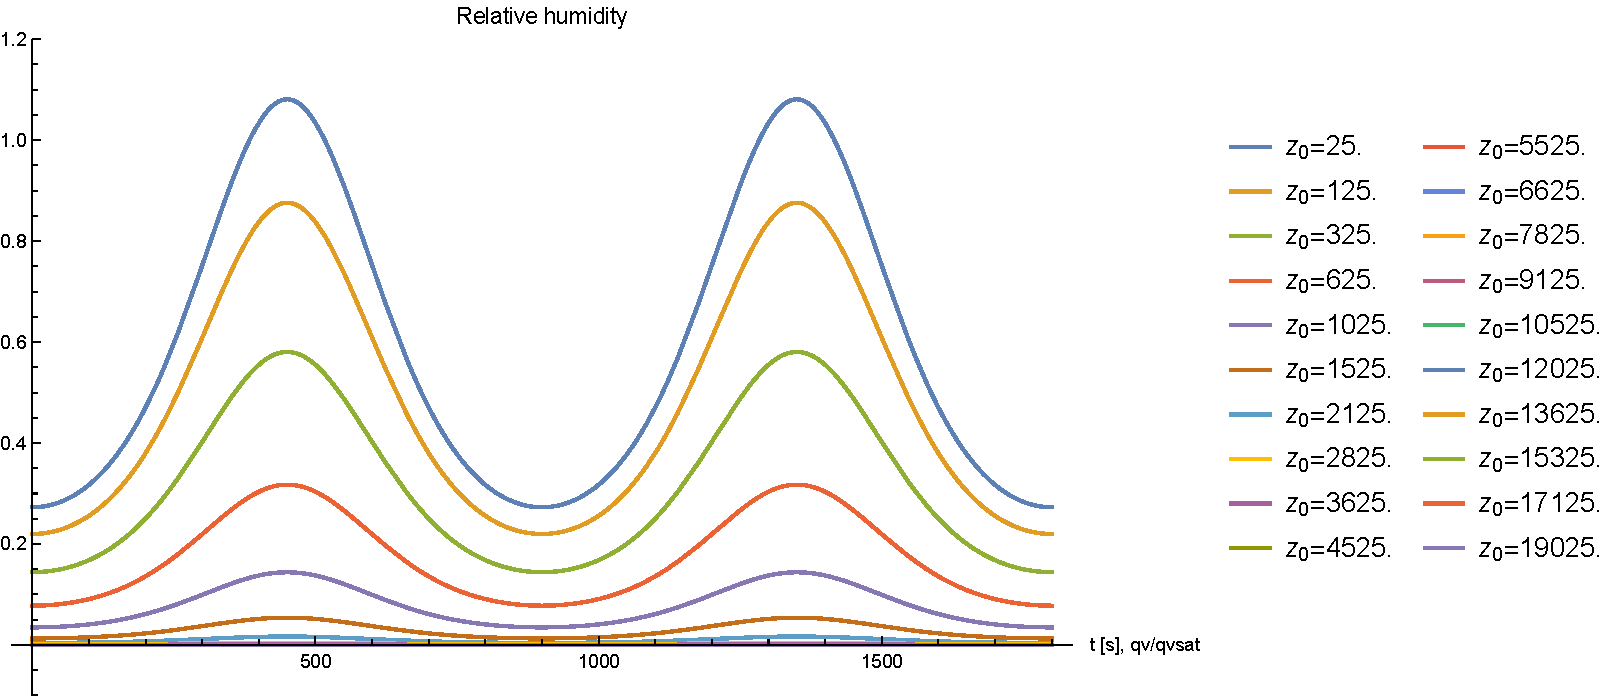
\includegraphics[width=\linewidth]{figures/relhumidity_plot}
\caption{Temperature for the same parameters as in Figures \ref{fig:geopotential},\ref{fig:density}, and \ref{fig:pressure}, with the additional parameters $q_{0}=6$E-3, $q_1=2.5$E-3.}\label{fig:humidity}
\end{figure}


\subsection{Time stepping}

The above dynamics are associated with the following \emph{tendencies}, the right-hand sides of \eqref{eq:geo_traj} and \eqref{eq:1d},
\begin{subequations}\label{eq:tends}
  \begin{align}
     \dot{w}(\phi,t) \equiv \totd{w}  &= \frac{2\pi w_0}{t_p}\sin\frac{\pi\phi}{gz_{top}}\cos\frac{2\pi t}{t_p} + \frac{\pi w_0^2}{2z_{top}}\sin\frac{2\pi\phi}{gz_{top}}\sin^2\frac{2\pi t}{t_p},\\
    \dot{\phi}(\phi,t) \equiv \totd{\phi} &= gw_0 \sin \frac{\pi \phi}{g z_{top}}\sin\frac{2\pi t}{t_p},\\
    \dot{\rho}(\phi, t, \rho) \equiv \totd{\rho} &= -\rho \frac{\pi w_0}{z_{top}}\cos\frac{\pi \phi}{g z_{top}}\sin\frac{2\pi t}{t_p},\\
    \dot{\theta_v} \equiv \totd{\theta_v} &= 0,\\
    \dot{q_v} \equiv \totd{q_v} &= 0.
  \end{align}
\end{subequations} 

%We use an explicit 2nd order Runge-Kutta method, hereafter RK2, for advancing \eqref{eq:column_dynamics} forward in time \cite[\S 8.3.3]{DahlquistBjork}.

%\paragraph{Case 1: Prescribed velocity.} In this case we assume that vertical velocity $w$ is prescribed by a known function $w=w(z,t)$, for example,
%\begin{equation}\label{eq:presc_velocity}
%  w(z,t) = w_0 \sin \frac{2\pi t}{t_p}\sin \frac{m \pi z}{z_{top}},
%\end{equation}
%where the user-chosen parameters are $w_0$, the maximum vertical velocity [m/s], $t_p$, the period [s], and $m$, the vertical wave number (a dimensionless integer).
%%Equations \eqref{eq:column_dynamics} are separable in this case and we can solve them analytically by recalling that $z = \phi/g$.
%Using \eqref{eq:presc_velocity} in \eqref{eq:column_dynamics} and recalling that $\phi = gz$, the geopotential equation becomes,
%\begin{equation}
%  \deriv{\phi}{t} = gw_0\sin\frac{2\pi t}{t_p}\sin\frac{m\pi \phi(t)}{g z_{top}},
%\end{equation}
%which is a separable equation for $\phi(t)$ that can be solved analytically for each interface.
%\begin{subequations}
%We find that
%\begin{equation}
%  \phi_{i+1/2}(t_{n+1}) = \frac{2 g z_{top}}{m \pi}\arccot\left[ {\exp\left(-\frac{m t_p w_0}{z_{top}}\sin^2\frac{\pi t_{n+1}}{t_p}\right)}{{\cot\left(\frac{m \pi \phi_0}{2gz_{top}}\right)}}\right],
%\end{equation}
%where $\phi_0 = \phi_{i+1/2}(0)$.
%Vertical velocity is updated as
%\begin{equation}
%  w_{i+1/2}(t_{n+1}) = w(\phi_{i+1/2}(t_{n+1})/g, t_{n+1}).
%\end{equation}
%
%The level variables lack source/sink terms; hence,
%\begin{align}
%  \partd{\pi}{s}_i(t_{n+1}) &= \partd{\pi}{s}_i(t_n),\\
%  \theta_{v,i}(t_{n+1}) &= \theta_{v,i}(t_{n+1}),\\
%  q_{v,i}(t_{n+1}) &= q_{v,i}(t_{n+1}).
%\end{align}
%
%Substituting \eqref{eq:presc_velocity} into the momentum equation we find that
%\begin{equation}
%  \mu_{i+1/2}(t_{n+1})= 1 + \frac{2\pi w_0}{gt_p}\cos\frac{2\pi t_{n+1}}{t_p}\sin\frac{m\pi \phi_{i+1/2}(t_{n+1})}{gz_{top}}.
%\end{equation}
%
%At each level we can directly apply the vertical derivative operator to get
%\begin{equation}
%  \partd{\phi}{s}_i(t_{n+1}) = \frac{\phi_{i+1/2}(t_{n+1})-\phi_{i-1/2}(t_{n+1})}{\Delta s_i}.
%\end{equation}
%After averaging the pseudodensity to the interfaces, the definition of $\mu$ gives $\partd{p}{s}$,
%\begin{equation}
%  \partd{p}{s}_{i+1/2}(t_{n+1}) = \mu_{i+1/2}(t_{n+1})\overline{\partd{\pi}{s}}_{i+1/2}(t_{n+1}).
%\end{equation}
%Pressure at the levels follows from the equation of state,
%\begin{equation}
%  p_{i+1}(t_{n+1}) = \exp\left(\frac{1}{{R}/{c_p}-1}\right)\left(\frac{\partd{\phi}{s}_ip_0^{R/c_p}}{R \theta_{v,i}(t_{n+1}) \partd{\pi}{s}_i(t_{n+1})}\right).
%\end{equation}
%Finally, surface pressure is updated as \cite[eqn.~(35)]{Taylor2020},
%\begin{equation}
%  p_s(t_{n+1}) = p_{top} -\frac{1}{2}\left[\left(\partd{p}{s}\Delta s\right)_{1/2} + \left(\partd{p}{s}\Delta s\right)_{n_{lev}+1/2}\right] + \sum_{k=0}^{n_{lev}}\left(\partd{p}{s}\Delta s\right)_{k+1/2}.
%\end{equation}
%\end{subequations}
%


\subsubsection{Simple microphysics}

A simple cloud model with warm-rain microphysics, often called \emph{Kessler microphysics}, is summarized in \cite[ch.~15]{RogersYau}.
It introduces mass mixing ratio tracers for cloud liquid water $q_c$ and rain water $q_r$ and is very similar to the microphysics used in \cite{SoongOgura1973,KlempWilhelmson1978}, and source terms for the dynamics equations.

\paragraph{Vertical velocity.} The vertical velocity $w$ is adjusted to account for falling liquid water, so that \eqref{eq:vert_vel} is now
\begin{equation*}
  \deriv{w}{t} = -g(1-\mu -(q_c+q_r)).  
\end{equation*}


\paragraph{Moisture variables.}
We assume, following \cite{SoongOgura1973,KlempWilhelmson1978}, that any supersaturated immediately condenses, and that any cloud liquid present in unsaturated air immediately evaporates.
Rain water only evaporates if $q_c = 0$.
These processes are represented by terms $E_1:q_v\leftrightarrow q_c$ and $E_2:q_v \leftarrow q_r$.
Equations \eqref{eq:theta_v} and \eqref{eq:q_v} become,
\begin{align}
  \deriv{\Theta}{t} &= \frac{L}{c_p \Pi }(E_1 + E_2), \\
  \deriv{q_v}{t} &= E_1 + E_2,
\end{align}
and new equations are added for $q_c$ and $q_r$:
\begin{align}
  \deriv{q_c}{t} &= -E_1 - (P_1 + P_2),\label{eq:cloud_water} \\
  \deriv{q_r}{t} &= -\frac{1}{\rho}\partd{}{z}(\rho q_r w_r) - E_2 + (P_1 + P_2), \label{eq:rain_water}
\end{align}
where $P_1:q_c+q_c\mapsto q_r$ and $P_2:q_c+q_r\mapsto q_r$ represent rain production from autoconversion and accretion, respectively, and $w_r$ is the velocity of rain water. Each is discussed below in greater detail.

Temperature $T$ and potential temperature $\theta$ are recovered from $\theta_v$ at level midpoints as
\begin{equation}\label{eq:temperature}
  T = \frac{\theta_v}{1+\alpha_v q_v} \left(\frac{p_0}{p}\right)^{-\kappa}, \quad \theta = \frac{\theta_v}{1+\alpha_vq_v},
\end{equation}
and 

  
\paragraph{Evaporation and condensation.}
The evaporation/condensation rate is parameterized by \cite[eqn.~(5)]{Srivastava1967}
\begin{equation}\label{eq:evap_param}
  E_1 = w\partd{q_v}{z}.
\end{equation}
Rain water is only allowed to evaporate in downdrafts and external to the cloud  \cite[eqn.~(10)]{Srivastava1967},
\begin{equation}\label{eq:rain_evap_param}
  E_2 = -\alpha_E w \partd{q_v}{z}, \quad \alpha_E = \begin{cases} 1 & w<0 \text{ and } q_c = 0,\\
 0 & \text{otherwise}  
 \end{cases}.
\end{equation}

\begin{rem}
Parameterizations \eqref{eq:evap_param} and \eqref{eq:rain_evap_param} are not meant to be interpreted as useful for physically realistic cloud simulations. 
They simply provide a basic model which is useful for testing purposes.
See \cite{SoongOgura1973,KlempWilhelmson1978} for more advanced parameterizations based on the difference between $q_v$ and the saturation mixing ratio, $q_{vs}$.
\end{rem}

\paragraph{Autoconversion.} Autoconversion only occurs in the presence of sufficient cloud water droplets.
Here, ``sufficient'' is defined as greater than a constant critical value, $q_c^{(crit)}$, and \cite[eqn.~(12)]{Srivastava1967}
\begin{equation}
  P_1 = \begin{cases}
    0 & q_c \le q_c^{(crit)}, \\
    \alpha_{auto}(q_c - q_c^{(crit)}) & q_c > q_c^{(crit)},
  \end{cases}
\end{equation}
where $\alpha_{auto}$ [1/s] is the inverse of the autoconversion time scale and $q_c^{(crit)}$ is a user-defined parameter.

\paragraph{Accretion.} Accretion describes the capture of cloud water droplets by rainwater droplets.
As in \cite{SoongOgura1973,KlempWilhelmson1978}, we use
\begin{equation}
  P_2 = \alpha_{accr}q_cq_r^{7/8},
\end{equation}
with $\alpha_{accr} = 2.2$.

\paragraph{Rainwater flux.} Rainwater by definition falls relative to the air; its vertical flux is described by the first term on the RHS of \eqref{eq:rain_water}.
  We use \cite[eqns.~(14),(15)]{SoongOgura1973} to approximate $w_r$,
  \begin{equation}
    w_r = 36.34 (\rho q_r)^{0.1364} ~\text{m/s}.
  \end{equation}
  

\subsection{Embedded parameterization}
